%!TEX program = xelatex
\documentclass[en,hazy,cyan,8pt,normal]{elegantnote}
\title{SUSTech - 25Fall - MAE5009 - Note}

\author{Yiyuan YING}
\institute{Southern University of Science and Technology}

% \version{2.50}
\date{\today}

\usepackage{array}
\usepackage{float}
\usepackage{microtype} % 微排版,通常能减少 underfull/overfull

\begin{document}

\maketitle

\section{Stress Analysis}
  \subsection{Stress State}
    \begin{itemize}
      \item Normal Stress
      \item Shear Stress
      \item Stress Transformation
    \end{itemize}

  \subsection{Equilibrium Equation of Stress}
    \begin{itemize}
      \item Body Force: Gravitational Force, Magnetic Force, Inertial Force
      \item Surface Force: Friction Force, Pressure, Viscous Force(Fluid Flow)
    \end{itemize}
    \begin{equation}\label{eq:001}
      Stress=\lim_{\Delta A \to 0} \frac{\Delta F}{\Delta A}
    \end{equation}
    The equation means the force at the per unit surface area. The unit is Pascal($Pa=N/m^2$).\\
    Other common units:
    \begin{itemize}
      \item $1 atm \approx 10^5 Pa = 0.1 MPa$
      \item $1 bar \approx 0.98 atm \approx 1 atm = 0.1 MPa$
    \end{itemize}
    Stress is a kind of tensor, different from \textbf{scalar} and \textbf{vector}.
    \begin{itemize}
      \item Scalar: only have magnitude, e.g. temperature, density;
      \item Vector: have both magnitude and direction, e.g. velocity, force;
      \item Tensor: magnitude and direction in multiple directions, e.g. stress, strain.
    \end{itemize}
    At a reference plane, the force $F$ is vertically upward, the normal stress $\sigma$ is perpendicular to the plane, while the shear stress $\tau$ is parallel to the plane.\\

  \subsection{2D Stress}
    \begin{figure}[H]
      \centering
      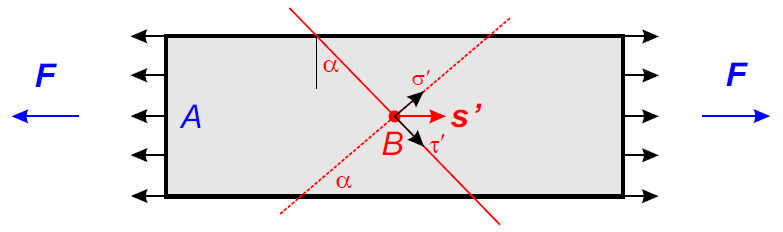
\includegraphics[width=0.6\textwidth]{image/001.png}
      \caption{Stress components on a reference plane}
      \label{fig:001}
    \end{figure}
    For the circumstances shown in Figure~\ref{fig:001}, the normal stress and shear stress on the reference plane can be determined.
    \begin{equation}\label{eq:002}
      A'=\frac{A}{\sin \alpha}, S=\frac{F}{A'}=\frac{F}{A} \sin \alpha,
      \begin{cases}
        \tau=S\cdot\cos\alpha=\frac{F}{A} \sin \alpha \cos \alpha\\
        \sigma=S\cdot\sin\alpha=\frac{F}{A} \sin^2 \alpha
      \end{cases}
    \end{equation}

  \subsection{3D Stress}
    \begin{figure}[H]
      \centering
      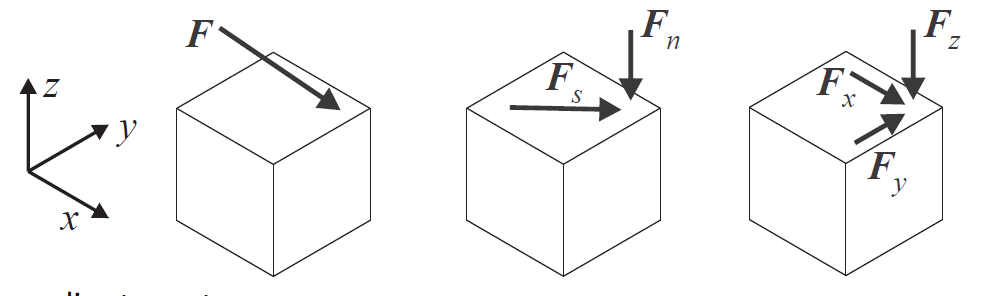
\includegraphics[width=0.6\textwidth]{image/002.png}
      \caption{Decomposition of an external force$F$}
      \label{fig:002}
    \end{figure}
    As shown in Figure~\ref{fig:002}, the force $F$ applied at an arbitrary angle to the x-y plane can be resolved into a normal component $F_n$ and a shear component $F_s$. The shear component can be further decomposed into Cartesian components $F_x$ and $F_y$.
    \begin{figure}[H]
      \centering
      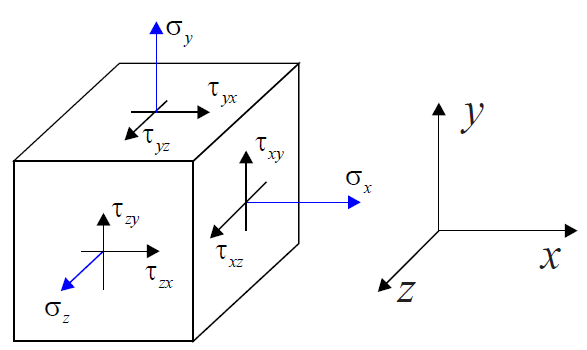
\includegraphics[width=0.6\textwidth]{image/003.png}
      \caption{Three-Dimensional State of Stress}
      \label{fig:003}
    \end{figure}
    As shown in the Figure~\ref{fig:003}, in every face has three stress components, with 1 normal stress($\sigma_x, \sigma_y, \sigma_z$) and 2 shear stresses($\tau_{xy}, \tau_{xz}, \tau_{yx}, \tau_{yz}, \tau_{zx}, \tau_{zy}$). Thus the components of stress can be expressed in a matrix form:
    \begin{equation}\label{eq:003}
      [\sigma]=
      \begin{bmatrix}
        \sigma_x & \tau_{xy} & \tau_{xz}\\
        \tau_{yx} & \sigma_y & \tau_{yz}\\
        \tau_{zx} & \tau_{zy} & \sigma_z
      \end{bmatrix}
    \end{equation}
    The sign convention is that normal stresses causing tension are positive, while those causing compression are negative.
    If we consider rotational equilibrium of the infinitesimal square shown as Figure~\ref{fig:004}, we can calculate the moment with respect to lower left corner:
    \begin{figure}[H]
      \centering
      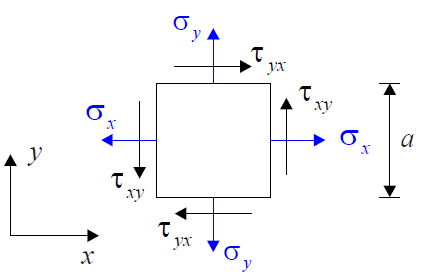
\includegraphics[width=0.4\textwidth]{image/004.png}
      \caption{Rotational Equilibrium of an Infinitesimal Element}
      \label{fig:004}
    \end{figure}
    \begin{equation}\label{eq:004}
      \sigma_x\cdot a (a/2)-\sigma_x\cdot a (a/2)+\sigma_y\cdot a (a/2)-\sigma_y\cdot a (a/2)+\tau_{xy}\cdot a \cdot a - \tau_{yx}\cdot a \cdot a=0
    \end{equation}
    Thus we have:
    \begin{equation}\label{eq:005}
      \tau_{xy}=\tau_{yx}
    \end{equation}
    Similarly, we can have:
    \begin{equation}\label{eq:006}
      \tau_{yz}=\tau_{zy}, \tau_{zx}=\tau_{xz}
    \end{equation}
    Which means, the stress matrix is symmetric, and there are 3 normal stresses and 3 shear stresses, totally 6 independent stress components in 3D stress state.
    \begin{equation}\label{eq:007}
      [\sigma]=
      \begin{bmatrix}
        \sigma_x & \tau_{xy} & \tau_{xz}\\
          & \sigma_y & \tau_{yz}\\
        Sym. &   & \sigma_z
      \end{bmatrix}
    \end{equation}

  \subsection{2D Stress Transformation}
    \begin{figure}[H]
      \centering
      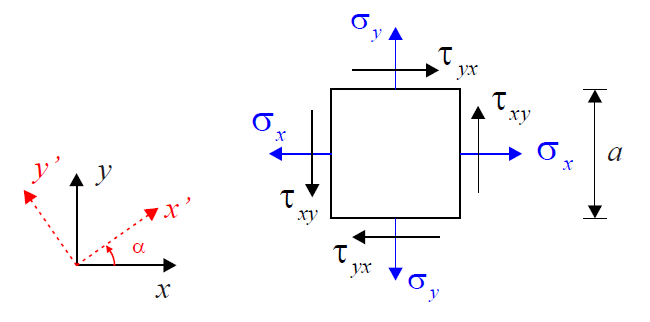
\includegraphics[width=0.6\textwidth]{image/005.png}
      \caption{Stress Transformation on an Arbitrary Plane}
      \label{fig:005}
    \end{figure}
    \begin{figure}[H]
      \centering
      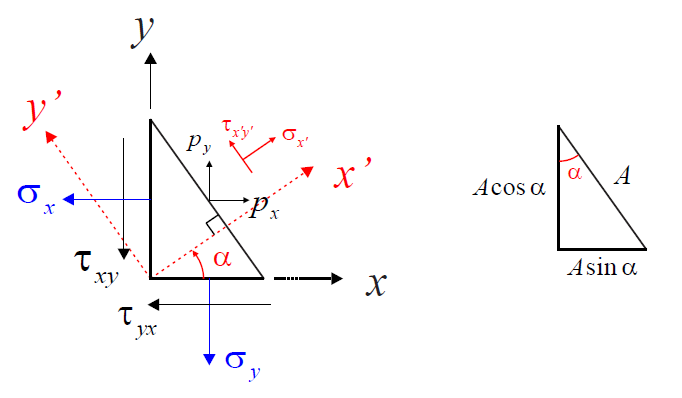
\includegraphics[width=0.6\textwidth]{image/006.png}
      \caption{Stress Components on an Inclined Plane in 2D Stress State}
      \label{fig:006}
    \end{figure}
    After the transformation shown in Figure~\ref{fig:005}, the new stress components are shown in Figure~\ref{fig:006}.
    The stress transformation equations may be derived based on force equilibrium analysis:
    \begin{equation}\label{eq:008}
      \sum F_x=0\Rightarrow p_x=\sigma_x\cos\alpha+\tau_{yx}\sin\alpha
    \end{equation}
    \begin{equation}\label{eq:009}
      \sum F_y=0\Rightarrow p_y=\sigma_y\sin\alpha+\tau_{xy}\cos\alpha
    \end{equation}
    Thus we have:
    \begin{equation}\label{eq:010}
      \begin{cases}
        \displaystyle \sigma_{x'}=\frac{\sigma_x+\sigma_y}{2}+\frac{\sigma_x-\sigma_y}{2}\cos2\alpha+\tau_{xy}\sin2\alpha\\
        \displaystyle \sigma_{y'}=\frac{\sigma_x+\sigma_y}{2}-\frac{\sigma_x-\sigma_y}{2}\cos2\alpha-\tau_{xy}\sin2\alpha\\
        \displaystyle \tau_{x'y'}=-\frac{\sigma_x-\sigma_y}{2}\sin2\alpha+\tau_{xy}\cos2\alpha
      \end{cases}
    \end{equation}
    In 2D circumstances, $\sigma'$ can be calculated by $\sigma'=\mathbf{R}\sigma \mathbf{R}^T$, in which:
    \begin{equation}\label{eq:011}
      \sigma=
      \begin{bmatrix}
        \sigma_x & \tau_{yx}\\
        \tau_{xy} & \sigma_y
      \end{bmatrix}, 
      \mathbf{R}=
      \begin{bmatrix}
        \cos\alpha & \sin\alpha\\
        -\sin\alpha & -\cos\alpha
      \end{bmatrix},
      \sigma'=
      \begin{bmatrix}
        \sigma_x' & \tau_{yx}'\\
        \tau_{xy}' & \sigma_y'
      \end{bmatrix}
    \end{equation}
    Also, the rotation angle $\alpha$ (principle directions)can be calculated by:
    \begin{equation}\label{eq:012}
      \tan2\alpha=\frac{2\tau_{xy}}{\sigma_x-\sigma_y}(\alpha\in[0,\pi])
    \end{equation}
    \begin{equation}\label{eq:013}
      \sin2\alpha=\pm\frac{2\tau_{xy}}{\sqrt{4\tau_{xy}^2+(\sigma_x-\sigma_y)^2}}, \quad \cos2\alpha=\frac{\sigma_x-\sigma_y}{\sqrt{4\tau_{xy}^2+(\sigma_x-\sigma_y)^2}}
    \end{equation}
    The principle stress can be calculated by:
    \begin{equation}\label{eq:014}
      \sigma_{1}=\frac{\sigma_x+\sigma_y}{2} + \sqrt{\left(\frac{\sigma_x-\sigma_y}{2}\right)^2+\tau_{xy}^2}
    \end{equation}
    \begin{equation}\label{eq:015}
      \sigma_{2}=\frac{\sigma_x+\sigma_y}{2} - \sqrt{\left(\frac{\sigma_x-\sigma_y}{2}\right)^2+\tau_{xy}^2}
    \end{equation}
    \begin{equation}\label{eq:016}
      \tau_{x'y'max}=\pm\sqrt{\left(\frac{\sigma_x-\sigma_y}{2}\right)^2+\tau_{xy}^2}
    \end{equation}
  
  \subsection{Mohr's circle of stress}
    \begin{figure}[H]
      \centering
      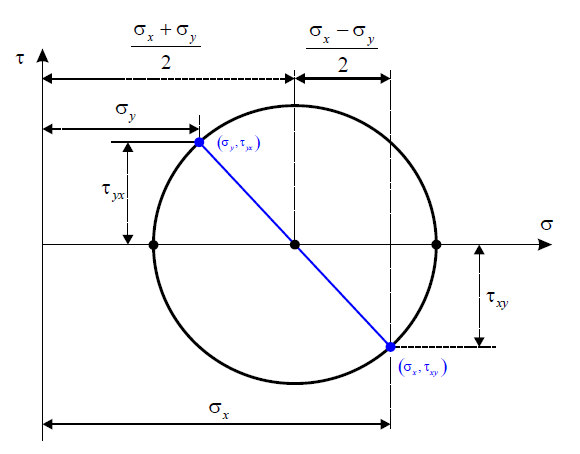
\includegraphics[width=0.6\textwidth]{image/007.png}
      \caption{Mohr's Circle of Stress}
      \label{fig:007}
    \end{figure}
    As shown in the Figure~\ref{fig:007}, 2D stress transformation can also be conveniently represented graphically in a circle. And from Equation~\ref{eq:010}, we can calculate that the equation of the circle is:
    \begin{equation}\label{eq:017}
      \left( \sigma - \frac{\sigma_x + \sigma_y}{2} \right)^2 + \tau^2 = \left( \frac{\sigma_x - \sigma_y}{2} \right)^2 + \tau_{xy}^2
    \end{equation}
    From the Equation~\ref{eq:017} we can get the center is $\displaystyle \left(\frac{\sigma_x + \sigma_y}{2}, 0\right)$ and the radius is $\displaystyle R=\sqrt{\left( \frac{\sigma_x - \sigma_y}{2} \right)^2 + \tau_{xy}^2}$.
    \begin{figure}[H]
      \centering
      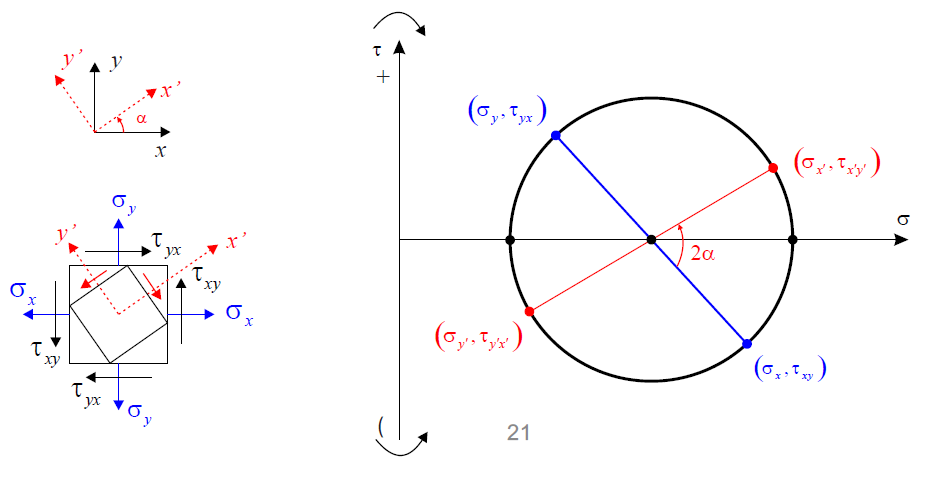
\includegraphics[width=0.6\textwidth]{image/008.png}
      \caption{Rotation in the Mohr's Circle of Stress}
      \label{fig:008}
    \end{figure}
    After rotating the x-y axis as shown in the Figure~\ref{fig:008}, the stress would be:
    \begin{equation}\label{eq:018}
      \begin{cases}
        \displaystyle \sigma_x'=\frac{\sigma_1+\sigma_2}{2}+\frac{\sigma_1-\sigma_2}{2}\cos2\alpha\\
        \displaystyle \sigma_y'=\frac{\sigma_1+\sigma_2}{2}-\frac{\sigma_1-\sigma_2}{2}\cos2\alpha\\
        \displaystyle \tau_{x'y'}=-\frac{\sigma_1-\sigma_2}{2}\sin2\alpha
      \end{cases}
    \end{equation}
  
  \subsection{3D stress transformation}
    Same to 2D stress transformation, the 3D stress transformation can also be expressed in matrix form:
    \begin{equation}\label{eq:019}
      \sigma'=\mathbf{R}\sigma \mathbf{R}^T
    \end{equation}
    where
    \begin{equation}\label{eq:020}
      \mathbf{R} =
        \begin{bmatrix}
        a_{11} & a_{12} & a_{13} \\
        a_{21} & a_{22} & a_{23} \\
        a_{31} & a_{32} & a_{33}
        \end{bmatrix}
        =
        \begin{bmatrix}
        \cos(x', x) & \cos(x', y) & \cos(x', z) \\
        \cos(y', x) & \cos(y', y) & \cos(y', z) \\
        \cos(z', x) & \cos(z', y) & \cos(z', z)
        \end{bmatrix}
    \end{equation}
    which means the direction cosines between the old and new coordinate axes.
    And in each columns and rows of matrix $\mathbf{R}$, we have:
    \begin{equation}\label{eq:021}
      a_{1i}^2 + a_{2i}^2 + a_{3i}^2 = 1, \quad i=1,2,3
    \end{equation}
    \begin{equation}\label{eq:022}
      a_{i1}^2 + a_{i2}^2 + a_{i3}^2 = 1, \quad i=1,2,3
    \end{equation}

  \subsection{3D principal stress}
    For symmetric matrix $\mathbf{A}$, its eigenvalue and eigenvector satisfy:
    \begin{equation}\label{eq:023}
      \mathbf{A}\mathbf{v}=\lambda \mathbf{v}
    \end{equation}
    \begin{equation}\label{eq:024}
      (\mathbf{A}-\lambda \mathbf{I})\mathbf{v}=0
    \end{equation}
    As the equation has non-zero $\mathbf{v}$ if and only if:
    \begin{equation}\label{eq:025}
      |\mathbf{A}-\lambda \mathbf{I}|=0
    \end{equation}
    Then we have the \textbf{Characteristic Equation} for the principle stress(in Equation~\ref{eq:023} - Equation~\ref{eq:025}, the matrix $\mathbf{A}$ can be replaced by stress matrix $[\sigma]$):
    \begin{equation}\label{eq:026}
      \det(\mathbf{\sigma}-\lambda \mathbf{I})=0
    \end{equation}
    Expand the determinant, we have:
    \begin{equation}\label{eq:027}
      \lambda^3 - I_1 \lambda^2 + I_2 \lambda - I_3 = 0
    \end{equation}
    The invariants $I_1, I_2, I_3$ are \textbf{Stress Invariants}, which means they are independent of the coordinate system:
    \begin{equation}\label{eq:028}
      \begin{cases}
        I_1 = \sigma_x + \sigma_y + \sigma_z=\sigma_1 + \sigma_2 + \sigma_3\\
        I_2 = \sigma_x \sigma_y + \sigma_y \sigma_z + \sigma_z \sigma_x - \tau_{xy}^2 - \tau_{yz}^2 - \tau_{zx}^2 = \sigma_1 \sigma_2 + \sigma_2 \sigma_3 + \sigma_3 \sigma_1\\
        I_3 = \sigma_x \sigma_y \sigma_z + 2 \tau_{xy} \tau_{yz} \tau_{zx} - \sigma_x \tau_{yz}^2 - \sigma_y \tau_{zx}^2 - \sigma_z \tau_{xy}^2 = \sigma_1 \sigma_2 \sigma_3
      \end{cases}
    \end{equation}

  \subsection{Differential equation of equilibrium}
    \begin{figure}[H]
      \centering
      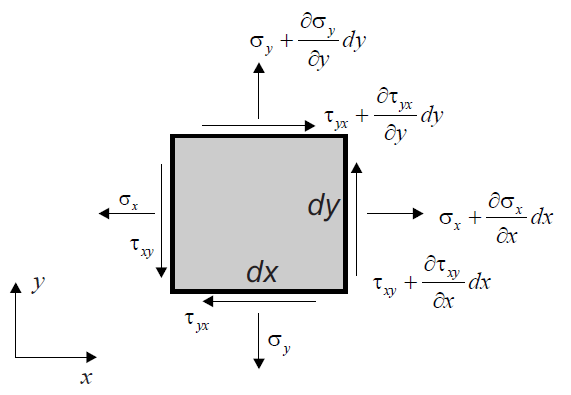
\includegraphics[width=0.6\textwidth]{image/009.png}
      \caption{Differential Element under Stress and Body Force}
      \label{fig:009}
    \end{figure}
    For the force balance $\sum F=0$ in the circumstances shown in Figure~\ref{fig:009}, we have:
    \begin{equation}\label{eq:029}
      \begin{cases}
        \displaystyle \frac{\partial\sigma_x}{\partial x}+\frac{\partial\tau_{yx}}{\partial y}+\frac{\partial\tau_{zx}}{\partial z}+f_x=0 \\
        \displaystyle \frac{\partial\tau_{xy}}{\partial x}+\frac{\partial\sigma_y}{\partial y}+\frac{\partial\tau_{zy}}{\partial z}+f_y=0 \\
        \displaystyle \frac{\partial\tau_{xz}}{\partial x}+\frac{\partial\tau_{yz}}{\partial y}+\frac{\partial\sigma_z}{\partial z}+f_z=0 &
      \end{cases}
    \end{equation}
    Which can be expressed like:
    \begin{equation}\label{eq:030}
      \nabla \cdot \sigma + f = 0
    \end{equation}
    In the Equation~\ref{eq:029} and Equation~\ref{eq:030}, $f$ is the body force intensities(per unit volume), e.g. gravitational force, magnetic force, inertial force.\\
    And when the body has acceleration, the Equation~\ref{eq:030} can be expressed as:
    \begin{equation}\label{eq:031}
      \nabla \cdot \sigma + f = \rho \frac{\partial^2 u}{\partial t^2}
    \end{equation}
    And for the torque balance $\sum M=0$ in the circumstances shown in Figure~\ref{fig:009}, we have:
    \begin{equation}\label{eq:032}
        \tau_{xy}=\tau_{yx}, \tau_{yz}=\tau_{zy}, \tau_{zx}=\tau_{xz}
    \end{equation}
    From the Equation~\ref{eq:029}, there are 6 independent unkowns in total, while only 3 equations. Thus additional equations are needed to complete the solutions of the stress distribution in a body. For example, Strain-displacement, Generalized Hooke's Law, etc.

\section{Strain Analysis}


\end{document}
